% SC2002 --- Chapter 1: Objects & Abstraction (0->100 ground-up)
\chapter{Objects \& Abstraction: Thinking in Objects}
\label{ch:objects}

\begin{quote}
\emph{``Object-oriented design is the art of deciding what to hide.''} --- Before syntax, we must learn to \emph{see} a system as cooperating objects. This chapter builds that lens from zero: what an object is, why abstraction matters, and how to decompose a problem without writing a line of Java yet.
\end{quote}

\noindent\fbox{\parbox{\dimexpr\linewidth-2\fboxsep-2\fboxrule}{%
\textbf{From zero: no SC1003/SC1007 assumed.} We define everything---programs, state, behaviour, abstraction---from first principles. No prior OOP or Java is assumed. Later chapters depend only on what is built here.}}

\section*{Learning Outcomes}
After this chapter you will be able to:
\begin{enumerate}[label=(L\arabic*)]
    \item define \emph{object}, \emph{state}, \emph{behaviour}, \emph{identity} and distinguish objects from values;
    \item explain abstraction, encapsulation boundaries, and decomposition via responsibility assignment;
    \item contrast procedural (verb-first) vs.\ object-oriented (noun-first) modelling on the same requirement;
    \item describe object interaction as \emph{message passing} and identify collaborators and responsibilities (CRC);
    \item apply abstraction criteria (cohesion, level, information hiding) to judge a proposed model.
\end{enumerate}

% ============================================================
\section{Why Objects? From Messy Reality to Manageable Models}
\label{sec:why-objects}
A program solves a real-world problem (library loans, ride-hailing, pixel rendering). Reality is messy: thousands of details, people, rules. An \emph{abstraction} keeps only the details relevant to the problem and hides the rest. An \emph{object} is the unit we use to do this.

Intuition first---picture a vending machine. You see buttons, a coin slot, a tray. You do not see the internal motors. The visible surface is the abstraction; the hidden motors are the implementation. Good objects are like that: a clear surface, a hidden interior.

\begin{figure}[h]
\centering
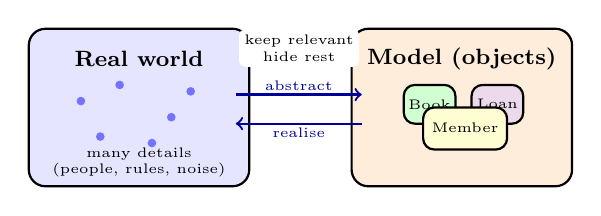
\begin{tikzpicture}[scale=0.82, every node/.style={font=\scriptsize}]
\node[draw,thick,fill=blue!10,rounded corners=6pt,minimum width=2.8cm,minimum height=2.0cm] (real) at (0,0) {};
\node[font=\footnotesize\bfseries] at (0,0.75) {Real world};
\foreach \x/\y in {-0.9/0.1, -0.3/0.35, 0.5/-0.15, 0.8/0.25, -0.6/-0.45, 0.2/-0.55} \fill[blue!55] (\x,\y) circle (1.9pt);
\node[font=\tiny,align=center] at (0,-0.85) {many details\\(people, rules, noise)};
\node[draw,thick,fill=orange!14,rounded corners=6pt,minimum width=2.8cm,minimum height=2.0cm] (model) at (5.0,0) {};
\node[font=\footnotesize\bfseries] at (5.0,0.75) {Model (objects)};
\draw[thick,fill=green!18,rounded corners=4pt] (4.1,-0.25) rectangle (4.9,0.35);
\node[font=\tiny,align=center] at (4.5,0.05) {Book};
\draw[thick,fill=violet!15,rounded corners=4pt] (5.15,-0.25) rectangle (5.95,0.35);
\node[font=\tiny,align=center] at (5.55,0.05) {Loan};
\draw[thick,fill=yellow!18,rounded corners=4pt] (4.4,-0.65) rectangle (5.7,0.0);
\node[font=\tiny,align=center] at (5.05,-0.32) {Member};
\draw[->,thick,blue!60!black] (1.5,0.2) -- (3.45,0.2) node[midway,above,font=\tiny,fill=white,inner sep=1pt] {abstract};
\draw[->,thick,blue!60!black] (3.45,-0.25) -- (1.5,-0.25) node[midway,below,font=\tiny,fill=white,inner sep=1pt] {realise};
\node[font=\tiny,align=center,fill=white,rounded corners=2pt,inner sep=2pt] at (2.48,0.92) {keep relevant\\hide rest};
\end{tikzpicture}
\caption{Abstraction selects relevant details from reality and packages them as objects (Book, Member, Loan).}
\label{fig:abstraction-filter}
\end{figure}

\begin{definition}[Abstraction]
An \emph{abstraction} is a simplified representation that retains properties relevant to a purpose and suppresses irrelevant detail. Good abstractions have high \emph{cohesion} (one purpose) and low \emph{coupling} (few dependencies). Abstraction is not vague---it is selective.
\end{definition}

% --- TikZ 2: Object = identity + state + behaviour ---
\begin{figure}[h]
\centering
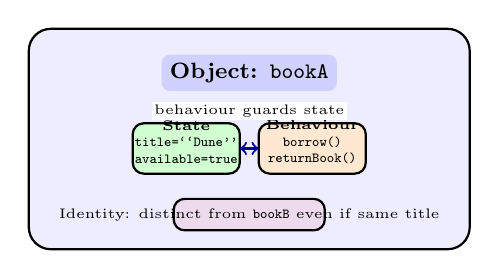
\begin{tikzpicture}[scale=0.80, every node/.style={font=\scriptsize}]
\node[draw,thick,fill=blue!7,rounded corners=8pt,minimum width=5.6cm,minimum height=2.8cm] (obj) at (0,0) {};
\node[font=\footnotesize\bfseries,fill=blue!18,rounded corners=3pt,inner sep=3pt] at (0,1.05) {Object: \texttt{bookA}};
\draw[thick,fill=green!18,rounded corners=4pt] (-1.85,0.25) rectangle (-0.15,-0.55);
\node[font=\tiny,align=center] at (-1.0,-0.05) {\textbf{State}\\\texttt{title=``Dune''}\\\texttt{available=true}};
\draw[thick,fill=orange!18,rounded corners=4pt] (0.15,0.25) rectangle (1.85,-0.55);
\node[font=\tiny,align=center] at (1.0,-0.05) {\textbf{Behaviour}\\\texttt{borrow()}\\\texttt{returnBook()}};
\draw[thick,fill=violet!14,rounded corners=4pt] (-1.2,-0.95) rectangle (1.2,-1.45);
\node[font=\tiny] at (0,-1.2) {Identity: distinct from \texttt{bookB} even if same title};
\draw[<->,thick,blue!60!black] (-0.15,-0.15) -- (0.15,-0.15);
\node[font=\tiny,fill=white,inner sep=1pt] at (0,0.45) {behaviour guards state};
\end{tikzpicture}
\caption{Every object has \emph{identity} (which object), \emph{state} (fields), and \emph{behaviour} (methods). Behaviour is the only way to observe or change state.}
\label{fig:object-anatomy}
\end{figure}

\begin{definition}[Object, State, Behaviour, Identity]
An \emph{object} is an encapsulated entity with (i) \emph{identity} (a distinct existence; two objects with equal fields are not the same object), (ii) \emph{state} (the values of its attributes at a moment), and (iii) \emph{behaviour} (operations it can perform, typically by reading/writing its state and collaborating with others).
\end{definition}

Values vs.\ objects: \texttt{42} and \texttt{"hi"} are \emph{values}---no identity beyond equality. A \texttt{Book} or \texttt{BankAccount} is an object---identity matters (your account $\neq$ my account even with same balance). Confusing the two is a common early error.

\section{Abstraction, Decomposition, Responsibility}
\label{sec:abstraction}
To design is to decompose. Given ``build a library system,'' we ask: what \emph{things} exist, what does each \emph{know} and \emph{do}, and who does it \emph{talk to}?

A classic lightweight tool is \textbf{CRC cards} (Class--Responsibility--Collaborator): for each candidate object write its responsibilities (what it must achieve) and collaborators (who it needs). Example: \texttt{Loan} --- responsibility ``track due date, detect overdue'' --- collaborators \texttt{Book}, \texttt{Member}.

\begin{example}[Library decomposition---first cut]
Nouns in the brief: \emph{Book, Member, Loan, Librarian}. Verbs: \emph{borrow, return, reserve, fine}. Candidate objects: \texttt{Book} knows its availability; \texttt{Loan} knows its due date; \texttt{Member} knows its loans. Librarian is an \emph{actor} (human), not necessarily an object---model what the system must remember, not every person in the world.
\end{example}

Information hiding: each object publishes an \emph{interface} (what you may ask it) and hides its representation (how it stores it). That lets us change one object's internals without breaking callers---the payoff of abstraction.

\subsection{Levels of Abstraction}
Abstractions nest. At the top, ``Library lends Books.'' One level down, ``Loan has a due date, Member has a borrowing limit.'' Further down, ``Due date is a \texttt{LocalDate}.'' Each level hides detail of the one below. Jumping levels (e.g., calculating fine inside UI code) breaks encapsulation and scatters knowledge.

\subsection{Cohesion and Coupling as Judges}
\emph{Cohesion} asks ``does this object do one thing well?'' A \texttt{LoanCalculator+Printer+Saver} class has low cohesion. \emph{Coupling} asks ``how many others does this object depend on?'' High coupling means one change ripples everywhere. Prefer many cohesive, loosely coupled objects over one god object.

% --- TikZ 3: Message passing between objects ---
\begin{figure}[h]
\centering
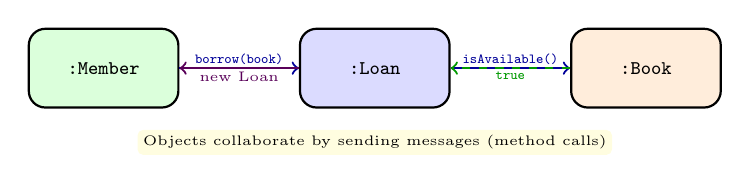
\begin{tikzpicture}[scale=0.82, every node/.style={font=\scriptsize}]
\node[draw,thick,fill=green!14,rounded corners=6pt,minimum width=1.9cm,minimum height=1.0cm] (m) at (0,0) {\texttt{:Member}};
\node[draw,thick,fill=blue!14,rounded corners=6pt,minimum width=1.9cm,minimum height=1.0cm] (l) at (4.2,0) {\texttt{:Loan}};
\node[draw,thick,fill=orange!14,rounded corners=6pt,minimum width=1.9cm,minimum height=1.0cm] (b) at (8.4,0) {\texttt{:Book}};
\draw[->,thick,blue!60!black] (m) -- (l) node[midway,above,font=\tiny,fill=white,inner sep=1pt] {\texttt{borrow(book)}};
\draw[->,thick,blue!60!black] (l) -- (b) node[midway,above,font=\tiny,fill=white,inner sep=1pt] {\texttt{isAvailable()}};
\draw[->,thick,green!60!black,dashed] (b) -- (l) node[midway,below,font=\tiny,fill=white,inner sep=1pt] {\texttt{true}};
\draw[->,thick,violet!70!black] (l) -- (m) node[midway,below,font=\tiny,fill=white,inner sep=1pt] {new Loan};
\node[font=\tiny,align=center,fill=yellow!12,rounded corners=2pt,inner sep=2pt] at (4.2,-1.15) {Objects collaborate by sending messages (method calls)};
\end{tikzpicture}
\caption{Message passing: a \texttt{Member} asks to borrow; the \texttt{Loan} checks the \texttt{Book}'s availability before creation.}
\label{fig:message-passing}
\end{figure}

\begin{remark}[Procedural vs.\ OO---verb-first vs.\ noun-first]
Procedural: ``steps to borrow a book'' --- one procedure reads/writes global arrays. OO: ``which object should be responsible for what?'' --- \texttt{Book} guards availability, \texttt{Loan} guards dates, \texttt{Member} guards limits. When requirements change (``add reservations''), OO changes are local; procedural changes ripple. The shift is not syntax but where knowledge lives.
\end{remark}

\begin{lstlisting}[language=Java, caption={Procedural vs.\ OO sketch---same requirement, different homes for logic.}]
// Procedural (data + separate functions) -- logic scattered
boolean borrowBook(int bookId, int memberId) {
    if (!books[bookId].available) return false;
    if (memberLoans[memberId].size() >= MAX) return false;
    // ... update arrays directly -- invariants checked nowhere centrally
}
// OO (behaviour lives with data) -- each object guards its invariant
class Book { boolean isAvailable() { ... } void markBorrowed() { ... } }
class Member { boolean canBorrow() { return loans.size() < MAX; } }
class Loan { static Loan create(Member m, Book b) {
    if (!b.isAvailable() || !m.canBorrow()) throw new IllegalStateException();
    b.markBorrowed(); Loan ln = new Loan(m,b); m.addLoan(ln); return ln;
}}
\end{lstlisting}

\section{Abstraction Criteria and Common Pitfalls}
\label{sec:abstraction-criteria}
How do you judge an abstraction? Three tests:

\paragraph{1. Does it hide a design decision?} If the caller would need to change when you change representation, the abstraction leaks. Example: exposing \texttt{books: Book[]} forces callers to know it is an array; switching to a \texttt{Map<Isbn,Book>} breaks them. Hide behind \texttt{findByIsbn(Isbn)} instead.

\paragraph{2. Is it at a consistent level?} A \texttt{Library} method that both checks borrowing rules and formats a receipt mixes policy with presentation. Split levels: policy (\texttt{LoanPolicy}), persistence (\texttt{Repository}), presentation (\texttt{ReceiptFormatter}).

\paragraph{3. Can you state its invariant in one sentence?} ``A \texttt{Book} is available iff no active \texttt{Loan} references it'' is crisp. ``\texttt{Library} does everything'' states no invariant---a warning sign.

\begin{example}[Leaky abstraction---and the fix]
\begin{lstlisting}[language=Java, caption={Leaky vs.\ encapsulated---caller dependency on representation.}]
// Leaky: caller knows loans are a List and manipulates it directly
library.getLoans().add(new Loan(member, book)); // invariant not checked!
// Encapsulated: Library enforces the invariant
library.borrow(memberId, bookId); // checks availability, limit, creates Loan atomically
\end{lstlisting}
\end{example}

\begin{remark}[Noun-verb heuristic---use, then validate]
Underline nouns/verbs in the requirements to seed candidates, then validate each candidate with CRC: does it have a crisp responsibility and a small collaborator set? Discard candidates that are really attributes (\texttt{dueDate}) or roles (\texttt{borrower} is a \texttt{Member} playing a role).
\end{remark}

\subsection{Design Exercise: Warm-Up Decomposition}
Walk through a tiny system end-to-end to cement the method.

\paragraph{Requirement.} ``A vending machine sells snacks. Customers insert coins, select a snack, receive change.'' Nouns: \texttt{Customer}, \texttt{Coin}, \texttt{Snack}, \texttt{VendingMachine}, \texttt{Transaction}. Verbs: \texttt{insert}, \texttt{select}, \texttt{dispense}, \texttt{refund}. CRC first draft:
\begin{itemize}[itemsep=0.2em]
    \item \texttt{Snack}: knows price, stock; collaborator none.
    \item \texttt{VendingMachine}: knows inventory, coin store; collaborators \texttt{Snack, Transaction}.
    \item \texttt{Transaction}: knows amount paid, change due; collaborators \texttt{Coin}.
\end{itemize}
Notice \texttt{Customer} is an actor outside the system---no class needed unless we track customer accounts. The boundary (what is inside vs.\ outside) is the first design decision.

\begin{lstlisting}[language=Java, caption={CRC to code---one object per responsibility, no god class.}]
class Snack { private String name; private int priceCents; private int stock;
    boolean inStock(){ return stock>0; } void dispense(){ stock--; } }
class Transaction { private int paid, price;
    int changeDue(){ return paid - price; } boolean paidEnough(){ return paid>=price; } }
\end{lstlisting}
This two-object split already enforces an invariant: stock never goes negative because \texttt{dispense} is only called after an \texttt{inStock} check inside \texttt{VendingMachine}.

\subsection{Visual Summary: From Requirement to Objects}
The object-oriented workflow is iterative: (1) harvest nouns/verbs, (2) draft CRC cards, (3) sketch a class diagram, (4) walk through scenarios with sequence diagrams, (5) refine. Each step hides one level of detail so the next step can proceed without drowning.

\begin{center}
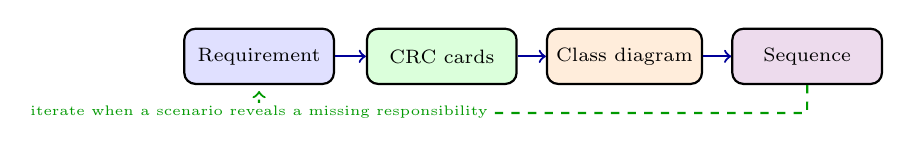
\begin{tikzpicture}[scale=0.80, every node/.style={font=\scriptsize}]
\node[draw,thick,fill=blue!12,rounded corners=4pt,minimum width=1.9cm,minimum height=0.7cm] (req) at (0,0) {Requirement};
\node[draw,thick,fill=green!14,rounded corners=4pt,minimum width=1.9cm,minimum height=0.7cm] (crc) at (2.9,0) {CRC cards};
\node[draw,thick,fill=orange!14,rounded corners=4pt,minimum width=1.9cm,minimum height=0.7cm] (cls) at (5.8,0) {Class diagram};
\node[draw,thick,fill=violet!14,rounded corners=4pt,minimum width=1.9cm,minimum height=0.7cm] (seq) at (8.7,0) {Sequence};
\draw[->,thick,blue!60!black] (req)--(crc); \draw[->,thick,blue!60!black] (crc)--(cls); \draw[->,thick,blue!60!black] (cls)--(seq);
\draw[->,thick,green!60!black,dashed] (seq) -- (8.7,-0.9) -- (0,-0.9) -- (0,-0.55) node[midway,below,font=\tiny,fill=white,inner sep=1pt] {iterate when a scenario reveals a missing responsibility};
\end{tikzpicture}
\end{center}
Iteration is the point---first drafts are wrong, and CRC/sequence walks are the cheapest way to discover it, before any Java is written.

\section{Chapter Notes}
Abstraction and information hiding are Parnas (1972); CRC cards are Beck \& Cunningham (1989). ``Message passing'' terminology is Smalltalk/Kay; Java/C++ realise it as method calls. Cohesion/coupling metrics originate with Constantine \& Yourdon. The noun-verb heuristic for finding objects is useful but fallible---always validate with responsibilities.

\section{Exercises}
\label{sec:ch01-exercises}
\begin{enumerate}[label=E1.\arabic*, leftmargin=*, itemsep=0.8em]
    \item \textbf{Object vs.\ value.} Give two domain examples where identity matters (must be objects) and two where only equality matters (values). What goes wrong if you model a value as an object and vice versa?
    \item \textbf{CRC drill.} For a ride-hailing app with \texttt{Rider, Driver, Trip, Payment}, write CRC cards (responsibilities + collaborators) for each. Which responsibilities, if misplaced, would create high coupling?
    \item \textbf{Abstraction quality.} A teammate models \texttt{Library} with one method \texttt{doEverything(String command)}. Diagnose using cohesion, coupling, and information hiding. Propose a refactored decomposition and justify each object's boundary.
    \item \textbf{Message trace.} Draw the message sequence for ``member returns a book late and incurs a fine.'' Show which object computes the fine and why---argue from responsibility assignment, not implementation convenience.
    \item \textbf{Procedural to OO.} Rewrite a procedural \texttt{transfer(fromId, toId, amount)} that manipulates a global \texttt{balances[]} array into an OO design with \texttt{Account} objects. Where does the invariant \texttt{balance $\ge$ 0} now live, and how is it preserved?
\end{enumerate}
% End of Chapter 1
